%  !TeX  root  =  user_guide.tex

\section{Модуль Текст с разделителями}\label{label_dltext}

% когда переработка раздела будет завершена,
% раскоментируйте следующую строку:
% \updatedisclaimer

Модуль <<Текст с разделителями>> позволяет вам добавить в QGIS текстовый файл
с разделителями как слой.

\minisec{Требования}

Для просмотра текстового файла с разделителями как слоя, данный файл должен
содержать:

\begin{enumerate}
\item Заголовок с названием полей. Заголовок должен быть первой строкой
в текстовом файле.
\item Заголовок должен включать поля X и Y. Эти поля могут иметь произвольное имя.
\item Координаты X и Y должны быть заданы как числа. При этом система
координат может быть любой.
\end{enumerate}

В качестве примера корректного текстового файла, приведем фрагмент файла
с данными высотных точек \filename{elevp.csv}, включенный в пробный набор
данных QGIS (см. Раздел~\ref{label_sampledata}):

\begin{verbatim}
X;Y;ELEV
-300120;7689960;13
-654360;7562040;52
1640;7512840;3
[...]
\end{verbatim}

Некоторые замечания по текстовому файлу:

\begin{enumerate}
\item В примере текстового файла используется разделитель \mbox{$;$}. В
качестве разделителя полей может быть использован любой символ.
\item Первая строка содержит заголовки столбцов. Она содержит поля X, Y и ELEV.
\item Не используйте кавычки ({\tt{}"{}}) для разделения полей.
\item Координата Х расположена в поле {\em X}.
\item Координата Y расположена в поле {\em Y}.
\end{enumerate}

\minisec{Использование модуля}
Перед использованием модуль должен быть включен, как это описано в
Разделе~\ref{sec:managing_plugins}.

Используйте кнопку \toolbtntwo{delimited_text}{Добавить слой из текста с разделителями}
на панели инструментов для открытия диалогового окна создания слоя из
текста с разделителями, общий вид которого приведен на Рисунке~\ref{fig:delim_text_plugin_dialog}.

\begin{figure}[ht]
   \centering
   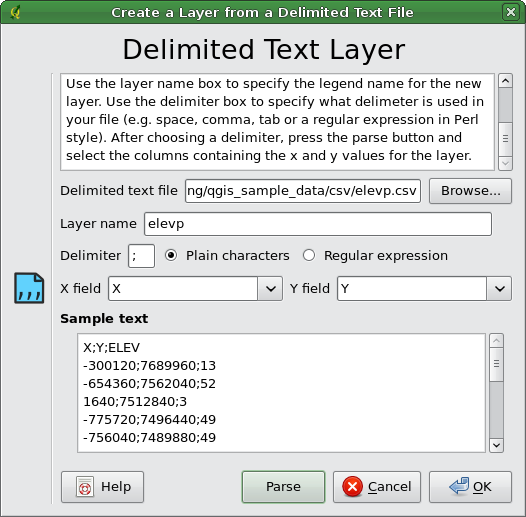
\includegraphics[clip=true, width=10cm]{delimited_text_dialog}
   \caption{Диалоговое окно <<Текст с разделителями>> \wincaption}\label{fig:delim_text_plugin_dialog}
\end{figure}

Сначала выберите файл для импорта (например, \filename{qgis\_sample\_data/csv/elevp.csv})
используя кнопку \button{ ... }. После того, как файл будет выбран, модуль
проведет анализ содержимого файла, используя текущий вариант символа
разделителя, в данном случае это символ (\mbox{$;$}). Для корректного
анализа файла важно указать правильный символ разделителя. Для указания
в качестве символа разделителя знака табуляции используйте
\mbox{$\backslash$}t (это регулярное выражение для символа табуляции).

После завершения анализа файла, выберите названия полей, содержащих
координаты X и Y, из раскрывающегося списка полей или укажите поле,
содержашее геометрию в формате WKT, и введя имя слоя
(например, \filename{elevp}), как показано на Рисунке~\ref{fig:delim_text_plugin_dialog}.
Для добавления слоя на карту нажмите кнопку \button{OK}. Текстовый файл
с разделителями теперь будет таким же, как любой другой слой в QGIS.

\FloatBarrier
